\documentclass[a4paper, 11pt]{article}
\usepackage{comment} % enables the use of multi-line comments (\ifx \fi) 
\usepackage{lipsum} %This package just generates Lorem Ipsum filler text. 
\usepackage{fullpage} % changes the margin
\usepackage[a4paper, total={7in, 10in}]{geometry}
\usepackage[fleqn]{amsmath}
\usepackage{amssymb,amsthm}  % assumes amsmath package installed
\newtheorem{theorem}{Theorem}
\newtheorem{corollary}{Corollary}
\usepackage{graphicx}
\usepackage{tikz}
\usetikzlibrary{arrows}
\usepackage{verbatim}
\usepackage[numbered]{mcode}
\usepackage{float}
\usepackage{tikz}
    \usetikzlibrary{shapes,arrows}
    \usetikzlibrary{arrows,calc,positioning}

    \tikzset{
        block/.style = {draw, rectangle,
            minimum height=1cm,
            minimum width=1.5cm},
        input/.style = {coordinate,node distance=1cm},
        output/.style = {coordinate,node distance=4cm},
        arrow/.style={draw, -latex,node distance=2cm},
        pinstyle/.style = {pin edge={latex-, black,node distance=2cm}},
        sum/.style = {draw, circle, node distance=1cm},
    }
\usepackage{xcolor}
\usepackage{mdframed}
\usepackage[shortlabels]{enumitem}
\usepackage{indentfirst}
\usepackage{hyperref}
    
\renewcommand{\thesubsection}{\thesection.\alph{subsection}}

\newenvironment{problem}[2][Problem]
    { \begin{mdframed}[backgroundcolor=gray!20] \textbf{#1 #2} \\}
    {  \end{mdframed}}

% Define solution environment
\newenvironment{solution}
    {\textit{Solution:}}
    {}

\renewcommand{\qed}{\quad\qedsymbol}
%%%%%%%%%%%%%%%%%%%%%%%%%%%%%%%%%%%%%%%%%%%%%%%%%%%%%%%%%%%%%%%%%%%%%%%%%%%%%%%%%%%%%%%%%%%%%%%%%%%%%%%%%%%%%%%%%%%%%%%%%%%%%%%%%%%%%%%%
\begin{document}
%Header-Make sure you update this information!!!!
\noindent
%%%%%%%%%%%%%%%%%%%%%%%%%%%%%%%%%%%%%%%%%%%%%%%%%%%%%%%%%%%%%%%%%%%%%%%%%%%%%%%%%%%%%%%%%%%%%%%%%%%%%%%%%%%%%%%%%%%%%%%%%%%%%%%%%%%%%%%%
\large\textbf{Ben Smith} \hfill \textbf{Problem Set - 2}   \\
Email: bxs566@case.edu \hfill ID: 3559750 \\
\normalsize Course: CSDS 337 - Compiler Design \hfill Term: Spring 2024\\
Instructor: Dr. Vipin Chaudhary \hfill Due Date: $14^{th}$ February, 2024 \\ \\
Number of hours delay for this Problem Set: \hfill 2\\
Cumulative number of hours delay so far: \hfill 26 \\ \\
I discussed this homework with: \hfill Jackson Schuetzle \\ \\
\underline{\bf SUBMISSION GUIDELINES:} Submit a zip file that includes the written answers and the flex file for Problem 4. \\

\noindent\rule{7in}{2.8pt}
%%%%%%%%%%%%%%%%%%%%%%%%%%%%%%%%%%%%%%%%%%%%%%%%%%%%%%%%%%%%%%%%%%%%%%%%%%%%%%%%%%%%%%%%%%%%%%%%%%%%%%%%%%%%%%%%%%%%%%%%%%%%%%%%%%%%%%%%
% Problem 1
%%%%%%%%%%%%%%%%%%%%%%%%%%%%%%%%%%%%%%%%%%%%%%%%%%%%%%%%%%%%%%%%%%%%%%%%%%%%%%%%%%%%%%%%%%%%%%%%%%%%%%%%%%%%%%%%%%%%%%%%%%%%%%%%%%%%%%%%
\begin{problem}{1 - 5 points}
Describe the language denoted by the following regular expression?

$(aa|bb)^*((ab|ba)(aa|bb)^*(ab|ba)(aa|bb)^*)^*$



\end{problem}
\begin{solution}
    This language is the set of all strings over the alphabet $\{a, b\}$ that contain an even number of $a$'s and an even number of $b$'s.

\end{solution}
\noindent\rule{7in}{2.8pt}

%%%%%%%%%%%%%%%%%%%%%%%%%%%%%%%%%%%%%%%%%%%%%%%%%%%%%%%%%%%%%%%%%%%%%%%%%
% Problem 2
%%%%%%%%%%%%%%%%%%%%%%%%%%%%%%%%%%%%%%%%%%%%%%%%%%%%%%%%%%%%%%%%%%%%%%%%%%%%%%%%%%%%%%%%%%%%%%%%%%%%%%%%%%%%%%%%%%%%%%%%%%%%%%%%%%%%%%%%

\begin{problem}{2 - 35 points}
Write regular definitions for the following languages:

\begin{enumerate}[a]
    \item All strings of lowercase letters that contain the five vowels in reverse order.
    \item Binary strings that has at least 3 characters, and the third character is 0.
    \item Binary strings that has number of 0s which is a multiple of 3
    \item Binary strings that starts and ends with the same character
    \item Binary strings that has odd length
    \item Binary strings that starts with 0 and has odd length, or starts with 1 and has even length
    \item Binary strings whose length is at least 1 and at most 3

\end{enumerate}

\end{problem}
\begin{solution}
    Your solutions go here
    \begin{enumerate}[a]
        \item   $\text{consonant} \longrightarrow ([bcd][fgh][j-n][p-t][v-z])^*a([bcd][fgh][j-n][p-t][v-z])$\\
              $\text{answer} \longrightarrow (\text{consonant})^*u^+(\text{consonant})^*o^+(\text{consonant})^*i^+(\text{consonant})^*e^+(\text{consonant})^*a^+$
        \item   $(0|1)(0|1)0(0|1)^*$
        \item   $(1^*01^*01^*01^*)^*$
        \item   $(0((0|1)^*0)?)|(1((0|1)^*1)?)$
        \item   $(1|0)((0|1)(0|1))^*$
        \item   $(0|(1(0|1)))((0|1)(0|1))^*$
        \item   $(0|1)(0|1)?(0|1)?$

    \end{enumerate}
\end{solution}
\noindent\rule{7in}{2.8pt}

%%%%%%%%%%%%%%%%%%%%%%%%%%%%%%%%%%%%%%%%%%%%%%%%%%%%%%%%%%%%%%%%%%%%%%%%%
% Problem 3
%%%%%%%%%%%%%%%%%%%%%%%%%%%%%%%%%%%%%%%%%%%%%%%%%%%%%%%%%%%%%%%%%%%%%%%%%%%%%%%%%%%%%%%%%%%%%%%%%%%%%%%%%%%%%%%%%%%%%%%%%%%%%%%%%%%%%%%%

\begin{problem}{3 - 10 points}
Provide transition diagram as an NFA to recognize the language represented by $a|abb|a^*b^+$. Convert this NFA to a DFA and show all steps.

\end{problem}

\begin{solution}
    \begin{figure}[H]
        \centering
        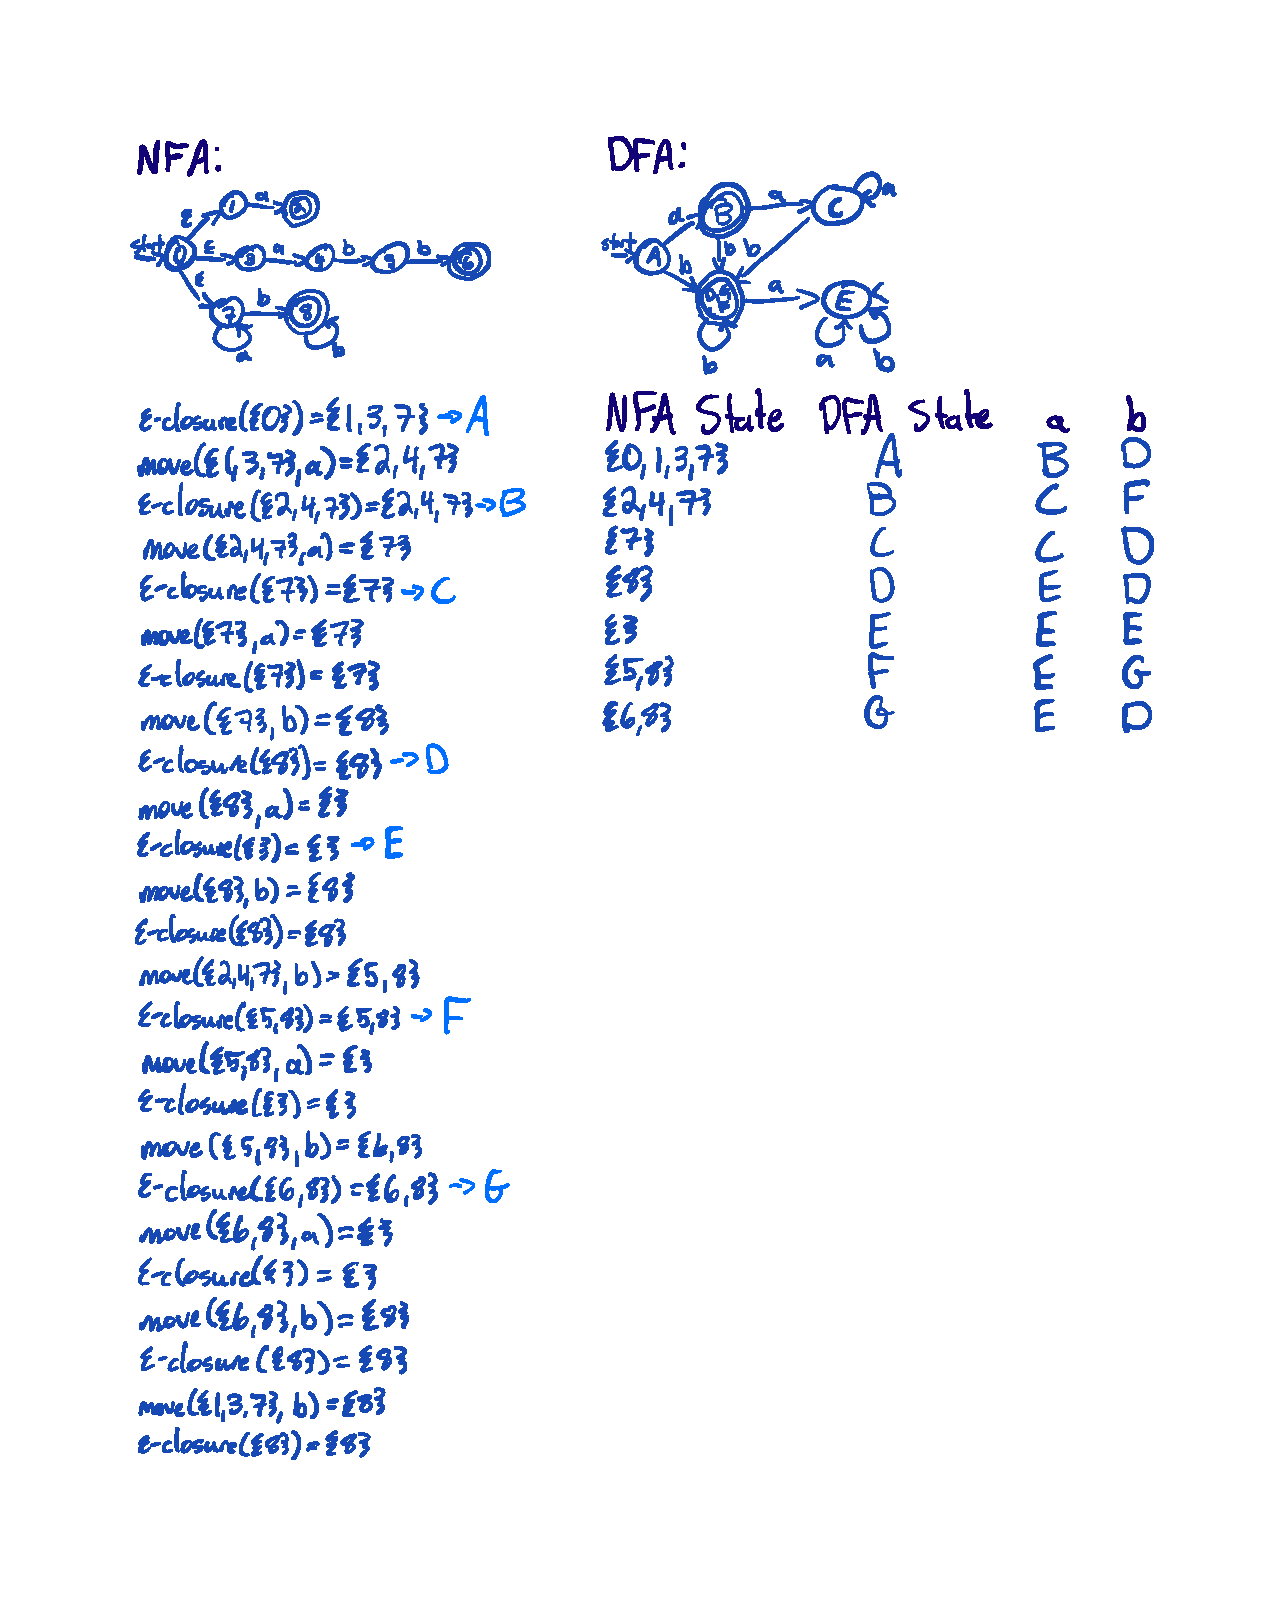
\includegraphics[scale=0.8]{Pset2.pdf}
        \caption{The NFA and DFA, with explanation.}
        \label{fig_2c}
    \end{figure}
\end{solution}

\noindent\rule{7in}{2.8pt}
%%%%%%%%%%%%%%%%%%%%%%%%%%%%%%%%%%%%%%%%%%%%%%%%%%%%%%%%%%%%%%%%%%%%%%%%%
%%%%%%%%%%%%%%%%%%%%%%%%%%%%%%%%%%%%%%%%%%%%%%%%%%%%%%%%%%%%%%%%%%%%%%%%%
% Problem 4
%%%%%%%%%%%%%%%%%%%%%%%%%%%%%%%%%%%%%%%%%%%%%%%%%%%%%%%%%%%%%%%%%%%%%%%%%%%%%%%%%%%%%%%%%%%%%%%%%%%%%%%%%%%%%%%%%%%%%%%%%%%%%%%%%%%%%%%%

\begin{problem}{4 - 50 points}
Write a flex program which does the following:
\begin{itemize}
    \item reads multiple input files
    \item for each file:
          \begin{itemize}
              \item it prints the number of characters, number words and number of lines
              \item it replaces more than one contiguous space by a single space
              \item it prints the number of single line C comments
              \item it prints the number of multiple line C comments
              \item it prints the number of occurrences of each of these keywords: $for$, $do$, and $while$
          \end{itemize}
    \item all the above counts are printed for each file in order and a cumulative number for all the files is also printed at the end
    \item the entire output is printed to a file named ``problem4output"
    \item the output should clearly indicate what each of the count indicates
    \item the flex file should be named ``problem4lex.l"
\end{itemize}
\end{problem}

\noindent\rule{7in}{2.8pt}

\end{document}
